\documentclass[style=smrt,mode=present,paper=screen]{powerdot}
% \documentclass[style=smrt,mode=handout,paper=letterpaper]{powerdot}

\usepackage{setspace}
\usepackage{listings}

\lstnewenvironment{code}{%
	\lstset{basicstyle=\tiny\ttfamily}
}{}

%\onehalfspacing

\title{\huge{\textbf{smrt Design Overview}} \\ \small{A 3D Media Center}}
\author {
	Cory Maccarrone
	\and
	Daniel Seikaly
	\and
	Evan Sheehan
	\and
	David Trowbridge
}
\date{December 13, 2005}
\begin{document}
\maketitle

\presenter{Daniel Seikaly}

% Overview slide.  Sort of a table of contents.
\begin{slide}[toc=,bm=]{Presentation Overview}
\tableofcontents[type=0,content=sections]
\end{slide}

% About the class
\section[slide=false]{The Class}
\begin{slide}{Senior Project Class}
\begin{itemize}
\item Year-long course
\item Required for all computer science sutdents at CU
\item Taught by Bruce Sanders
\item Offered every year since its inception in 1987
\item Since then 1140 students have finished 237 projects
\item \textit{smrt} is one of 15 projects involving 68 students
\item Other projects vary from card games to 3D image conversion tools
\item Its purpose is to give students "real world" experience
\end{itemize}
\end{slide}

\section{Project Overview}

% The Problem
\begin{slide}{The Problem}
\begin{itemize}
\item Current media center software designed in 2D
\item Can we benefit from a third dimension?
\begin{itemize}
	\item More efficient representation of data?
	\item More intuitive user interface?
	\item Eye candy
\end{itemize}
\end{itemize}
\end{slide}

% The "Solution"
\begin{slide}{The Solution: smrt}
\begin{itemize}
\item Media center application based on Sun's Looking Glass 3D
\begin{itemize}
	\item Framework for 3D interfaces
	\item Input device events
	\item Embedding external programs into the 3D environment
\end{itemize}
\item Provides TiVO-like functionality in a 3D environment
\item Capabilities for navigating through vast libraries of media
\begin{itemize}
	\item Categories
	\item Filesystem navigation
\end{itemize}
\item Play and record live TV, and play DVDs and music
\end{itemize}
\end{slide}

% Conceptual Diagram
\begin{slide}{Conceptual Diagram}
\begin{figure}[htb]
	\includegraphics[width=4in]{../lib/figures/conceptual_overview}
\end{figure}
\end{slide}

% Environmental Requirements
\begin{slide}{Environmental Requirements}
\begin{itemize}
\item Software Environment
\begin{itemize}
	\item Sun Java Development Kit version 5.0
	\item Latest version of Looking Glass 3D (currently 0.7.1)
\end{itemize}
\item Hardware Environment
\begin{itemize}
	\item TV/HDTV ``capable''
	\item Input from keyboard and (possibly) remote control
	\item Extensible to new and esoteric input devices
\end{itemize}
\end{itemize}
\end{slide}

% Functional Requirements
\begin{slide}{Functional Requirements}
\begin{itemize}
\item Display at multiple screen resolutions (NTSC and HDTV)
\item Provide mechanisms for displaying all available media
\begin{itemize}
	\item Local media (mp3s, etc.)
	\item DVDs, audio CDs
	\item Live TV
\end{itemize}
\item Schedule a TV program to record
\item User interface efficiency
\item Interface must utilize the third dimension
\end{itemize}
\end{slide}

\presenter{Cory Maccarrone}

\section{User Interface}

\begin{slide}{Ring Menu}
\begin{itemize}
\item Used for menus with few options
\item Requires at most $n \over 2$ clicks to reach an item
\item Selected item is biggest and in front
\end{itemize}
\begin{figure}[htb]
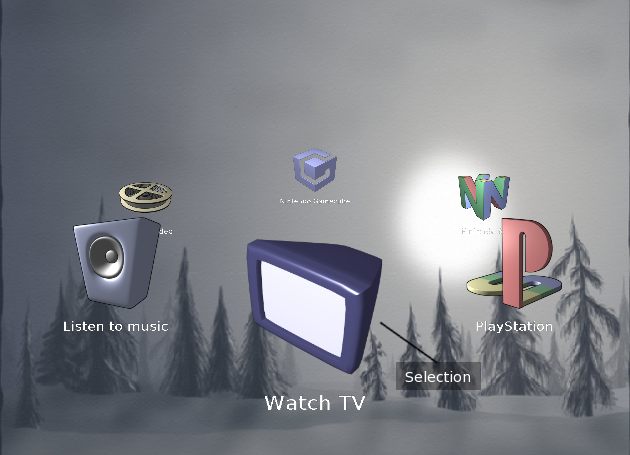
\includegraphics[width=2.5in]{../design/figures/ring_menu}
\end{figure}
\end{slide}

\begin{slide}{Arc Menu}
\begin{itemize}
\item Used for larger capacity menus
\item Not all items visible on the screen
\item Selected item is biggest and centered
\item Space for a preview area
\end{itemize}
\begin{figure}[htb]
\includegraphics[width=2.5in]{../design/figures/arc_menu}
\end{figure}
\end{slide}

\begin{slide}{Cityscape Menu}
\begin{itemize}
\item Used for filesystem and album browsing
\item Similar to the file browser in the movie \emph{Jurassic Park}
\item Files and directories, or albums and songs
\item Zooms in on directories
\end{itemize}
\begin{figure}[htb]
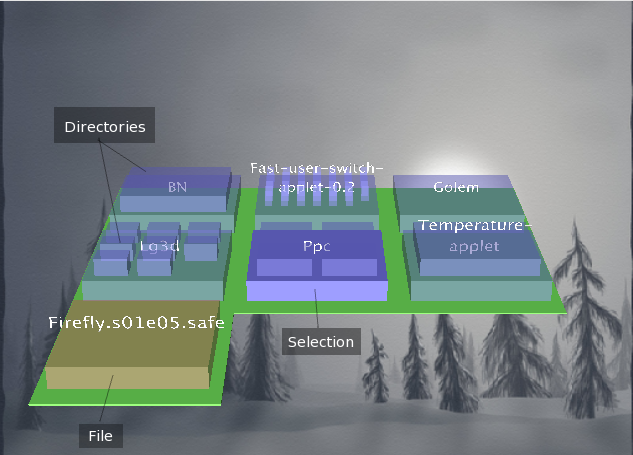
\includegraphics[width=2.5in]{../design/figures/city_menu}
\end{figure}
\end{slide}

\begin{slide}{Context Stack}
\begin{itemize}
\item Menus and applications are pushed onto a stack when they are opened,
      popped when application exits or menu is ``closed''
\item Bottom item on the stack can never be popped.
\item Menu based navigation is extremely intuitive and familiar
\item Equivalent to forward/back navigation in a web browser
\end{itemize}
\end{slide}

\presenter{David Trowbridge}

\begin{slide}{Example Session}
\begin{figure}[htb]
	\includegraphics[width=4in]{figures/example-session-01}
\end{figure}
\end{slide}

\begin{slide}[toc=,bm=]{Example Session, continued...}
\begin{figure}[htb]
	\includegraphics[width=4in]{figures/example-session-02}
\end{figure}
\end{slide}

\begin{slide}[toc=,bm=]{Example Session, continued...}
\begin{figure}[htb]
	\includegraphics[width=4in]{figures/example-session-03}
\end{figure}
\end{slide}

\begin{slide}[toc=,bm=]{Example Session, continued...}
\begin{figure}[htb]
	\includegraphics[width=4in]{figures/example-session-04}
\end{figure}
\end{slide}

\begin{slide}[toc=,bm=]{Example Session, continued...}
\begin{figure}[htb]
	\includegraphics[width=4in]{figures/example-session-05}
\end{figure}
\end{slide}

\begin{slide}[toc=,bm=]{Example Session, continued...}
\begin{figure}[htb]
	\includegraphics[width=4in]{figures/example-session-06}
\end{figure}
\end{slide}

\begin{slide}[toc=,bm=]{Example Session, continued...}
\begin{figure}[htb]
	\includegraphics[width=4in]{figures/example-session-07}
\end{figure}
\end{slide}

\begin{slide}[toc=,bm=]{Example Session, continued...}
\begin{figure}[htb]
	\includegraphics[width=4in]{figures/example-session-08}
\end{figure}
\end{slide}

\begin{slide}[toc=,bm=]{Example Session, continued...}
\begin{figure}[htb]
	\includegraphics[width=4in]{figures/example-session-09}
\end{figure}
\end{slide}

\begin{slide}[toc=,bm=]{Example Session, continued...}
\begin{figure}[htb]
	\includegraphics[width=4in]{figures/example-session-10}
\end{figure}
\end{slide}

\begin{slide}[toc=,bm=]{Example Session, continued...}
\begin{figure}[htb]
	\includegraphics[width=4in]{figures/example-session-11}
\end{figure}
\end{slide}

\presenter{Evan Sheehan}

\section{Software Modules}
\begin{slide}{Module Overview}
\begin{figure}
\includegraphics[width=3in]{../lib/figures/modular_overview}
\end{figure}
\end{slide}

\begin{slide}{State Controller}
\begin{itemize}
	\item Tracks state changes
	\item Stack of menus and applications (\emph{Context} objects)
	\item Passes LG3D events to the current \emph{Context}
\end{itemize}
\begin{figure}
\includegraphics[height=4in,angle=-90]{../lib/figures/MediaCenter-uml}
\end{figure}
\end{slide}

\begin{slide}{Menus}
\begin{itemize}
	\item Implements \emph{Context} interface
	\item Tracks items and responds to events
	\item Displays items on the screen
\end{itemize}
\begin{figure}[htb]
\includegraphics[height=3in,angle=-90]{../lib/figures/Menu-uml}
\end{figure}
\end{slide}

\begin{slide}{Application Manager}
\begin{itemize}
	\item Keeps track of all external applications, associates file types
	\item Sets up LG3D framework for X11 integration
\end{itemize}
\begin{figure}
\includegraphics[height=4in,angle=-90]{../lib/figures/MediaCenter-uml}
\end{figure}
\end{slide}

\begin{slide}{Application Factories}
\begin{itemize}
	\item Used to launch external applications
	\item One factory per application
	\item Keeps an array of regular expressions to match file extensions
\end{itemize}
\begin{figure}
\includegraphics[height=4in,angle=-90]{../lib/figures/ApplicationFactory-uml}
\end{figure}
\end{slide}

\begin{slide}{Applications}
\begin{itemize}
	\item Abstract class for each application
	\item Provides mechanisms for commands to be sent to applications
\end{itemize}
\begin{figure}
\includegraphics[height=4in, angle=-90]{../lib/figures/Application-uml}
\end{figure}
\end{slide}

\section{Classes}

\begin{slide}{StateController}
\begin{itemize}
\item StateController
\begin{itemize}
	\item \textbf{static StateController} getInstance ()
	\item \textbf{void} action (\textbf{String} \textit{action}, \textbf{String} \textit{arg})
	\item \textbf{void} push (\textbf{Context} \textit{context})
	\item \textbf{void} pop ()
	\item \textbf{void} pop (\textbf{Context} \textit{test})
\end{itemize}
\item Context
\begin{itemize}
	\item \textbf{void} ProcessEvent (\textbf{LgEvent} \textit{event})
\end{itemize}
\end{itemize}
\end{slide}

\begin{slide}{Application}
\begin{itemize}
\item application.Application
\begin{itemize}
	\item \textbf{void} run ()
\end{itemize}
\item application.ApplicationFactory
\begin{itemize}
	\item \textbf{public String}[] \textit{regexs}
	\item \textbf{Application} launch (\textbf{String} \textit{arg})
\end{itemize}
\item application.ApplicationManager
\begin{itemize}
\item \textbf{void} registerApplication (\textbf{ApplicationFactory} \textit{factory})
\item \textbf{Application} launch (\textbf{String} \textit{arg})
\end{itemize}
\end{itemize}
\end{slide}

\begin{slide}{Menu}
\begin{itemize}
\item menu.Menu
\begin{itemize}
	\item \textbf{void} addItem (\textbf{Item} \textit{item})
	\item \textbf{void} removeItem (\textbf{Item} \textit{item})
\end{itemize}
\item menu.Item
\begin{itemize}
	\item \textbf{void} activate ()
\end{itemize}
\end{itemize}
\end{slide}

\begin{slide}{CityScape}
\begin{itemize}
\item menu.FilesystemCity
\begin{itemize}
	\item \textbf{void} setFilters (\textbf{String}[] \textit{filters})
	\item \textbf{void} setRoot (\textbf{String} \textit{root})
\end{itemize}
\item menu.Directory
\begin{itemize}
	\item \textbf{void} setPath (\textbf{String} \textit{path})
	\item \textbf{String} getPath ()
	\item \textbf{void} createSubItems (\textbf{int} \textit{items})
	\item \textbf{void} realizeSublevel ()
\end{itemize}
\item menu.FilesystemCity.DirectoryCrawler
\begin{itemize}
	\item \textbf{void} run ()
\end{itemize}
\item menu.filter.FilenameFilter
\begin{itemize}
	\item \textbf{String} filter (\textbf{String} \textit{path}, \textbf{String} \textit{name})
\end{itemize}
\end{itemize}
\end{slide}

\presenter{David Trowbridge}

\section{File Formats}

\begin{slide}{Menu files}
\begin{itemize}
	\item Menus are referenced by filename -- loading ``main'' will use ``main.menu''
	\item Uses Java's XML serialization
	\item File contains one Menu object and any number of Item object
	\item Specialized menu types (such as FilesystemCity) can have special
	      configuration without upsetting other subsystems
\end{itemize}
\end{slide}

\begin{slide}[method=direct]{Example .menu}
\begin{code}
<java version="1.5.0" class="java.beans.XMLDecoder">
    <object class="org.jdesktop.lg3d.apps.smrt.menu.RingMenu"/>
    <object class="org.jdesktop.lg3d.apps.smrt.menu.IconItem">
        <void property="iconFilename">   <string>tv.png</string>   </void>
        <void property="label">          <string>Watch TV</string> </void>
        <void property="action">         <string>push</string>     </void>
        <void property="actionArgument"> <string>tv</string>       </void>
    </object>
    <object class="org.jdesktop.lg3d.apps.smrt.menu.IconItem">
        <void property="iconFilename">   <string>music.png</string> </void>
        <void property="label">
	    <string>Listen to Music</string>
	</void>
        <void property="action">         <string>push</string>      </void>
        <void property="actionArgument"> <string>music</string>     </void>
    </object>
</java>
\end{code}
\end{slide}

\begin{slide}{Applications Configuration}
\begin{itemize}
	\item Want to leverage any existing player applications
	\item Different players for different media types -- no existing player can do everything
	\item \textit{applications.conf} associates regular expressions with ApplicationFactory objects
	\item Regular expression is matched against the argument given to \textbf{launch} actions
\end{itemize}
\end{slide}

\begin{slide}[method=direct]{applications.conf}
\begin{code}
<java version="1.5.0" class="java.beans.XMLDecoder">
    <object class="org.jdesktop.lg3d.apps.smrt.application.XineFactory">
        <void property="regexs">
            <array class="java.lang.String">
                <string>.*\.avi</string>
                <string>.*\.mpeg</string>
                <string>dvd\://.*</string>
            </array>
        </void>
    </object>
    <object class="org.jdesktop.lg3d.apps.smrt.application.MPlayerFactory">
        <void property="regexs">
            <array class="java.lang.String">
                <string>tv\://p{Digit}*</string>
            </array>
        </void>
    </object>
</java>
\end{code}
\end{slide}

\presenter{Daniel Seikaly}

\section[slide=false]{Summary}
\begin{slide}[toc=,bm=]{Summary}
\tableofcontents[content=sections,type=1]
\end{slide}

\section[slide=false]{Questions?}
\begin{slide}[toc=,bm=]{Questions}
\begin{figure}[htb]
	\includegraphics[width=3in]{../lib/figures/fishstick}
\end{figure}
\end{slide}

\end{document}

